\documentclass[11pt,a4paper]{article}
\usepackage[utf8]{inputenc}
\usepackage[french]{babel}
\usepackage[T1]{fontenc}
\usepackage{amsmath}
\usepackage{amsfonts}
\usepackage{amssymb}
\usepackage{graphicx}
\usepackage{pdfpages}
\usepackage{epstopdf}
\usepackage{xcolor}
\usepackage[left=2cm,right=2cm,top=2cm,bottom=2cm]{geometry}
\title{SINF1121 - Groupe 9\\Rapport 1}
\author{Gégo Anthony\\Derval Guillaume}
\def\blurb{\textsc{Université catholique de Louvain\\
  École polytechnique de Louvain}}
\def\clap#1{\hbox to 0pt{\hss #1\hss}}%
\def\ligne#1{%
  \hbox to \hsize{%
    \vbox{\centering #1}}}%
\def\haut#1#2#3{%
  \hbox to \hsize{%
    \rlap{\vtop{\raggedright #1}}%
    \hss
    \clap{\vbox{\vfill\centering #2\vfill}}%
    \hss
    \llap{\vtop{\raggedleft #3}}}}%
\begin{document}
\begin{titlepage}
\thispagestyle{empty}\vbox to 1\vsize{%
  \vss
  \vbox to 1\vsize{%
    \haut{\includegraphics[scale=0.15]{logo_ucl.pdf}}{\blurb}{\includegraphics[scale=0.4]{logo_epl.jpg}}
    \vfill
    \ligne{\huge \textbf{\textsc{Systèmes informatiques II (INGI1113)}}}
    \vspace{5mm}
    \ligne{\Large \textbf{Projet 1 - Multiplication de matrices creuses}}
    \vspace{5mm}
    \ligne{\large{-- 6 octobre 2013 --}}
    \vfill
    \ligne{%
      \begin{tabular}{c}
        \textsc{Travail du groupe G35 :}
      \end{tabular}}
    \vspace{5mm}
    \ligne{%
      \begin{tabular}{lrclr}
         \textsc{Derval} Guillaume  & 68911100 & \hspace{80pt} & \textsc{Gégo} Anthony  & 28581100
      \end{tabular}
      }
    }%
  \vss
  }
\end{titlepage}

\section{Introduction}
En guise de premier projet pour le cours de Systèmes informatiques II, nous avons été invités à réaliser un petit programme de multiplication de matrices creuses. L'enjeu était de trouver une représentation de ces matrices afin de stocker uniquement les informations utiles et ainsi de simplifier les calculs.
La solution retenue est la représentation de Yale. Plusieurs tests de comparaison avec un produit matriciel classique ont été effectués et seront présentés par après.
\section{Représentation des matrices creuses}
Afin de représenter les matrices creuses de manière légère, nous avons opté pour la représentation de Yale\footnote{Voir : http://en.wikipedia.org/wiki/Sparse\_matrix\#Yale\_format}. Celle-ci consiste à mémoriser la valeurs des éléments non-nuls de la matrice avec leurs positions. 

Nous utilisons principalement une structure en liste chainée où un nœud contient la valeur de l'élément et l'indice de la colonne où il se trouve. Nous disposons également d'un tableau de pointeurs vers des nœuds, d'une taille identique au nombre de lignes de la matrice, où l'élément d'indice $i$ pointe vers le premier nœud/élément de la ligne $i$ de la matrice.

Une illustration de cette représentation est disponible à la figure \ref{matrix}.

\begin{figure}[h]
\centering
\includegraphics[scale=0.9]{matrix.pdf}
\caption{Représentation retenues pour les matrices}
\label{matrix}
\end{figure}

En raison de la structure choisie, le produit est dès lors réalisé ligne par ligne. Soit $M_1$ et $M_2$ deux matrices à multiplier pour donner $M_3$. Pour chaque ligne i de $M_1$, et pour chaque colonne j de $M_1$, le produit de la ligne j de $M_2$ multiplié par l'élément (i,j) de $M_1$ est ajouté à la ligne i de $M_3$. Pour plus de clarté, le déroulement étape par étape d'un produit est illustré à la figure \ref{produit}.

\begin{figure}[h]
\centering
\includegraphics[scale=0.6]{produit.pdf}
\caption{Étapes de réalisation du produit matriciel}
\label{produit}
\end{figure}

\section{Comparaison avec la méthode naïve}
Afin de démontrer l'efficacité de la méthode mise en place par rapport à la méthode naïve de multiplication matricielle (où les valeurs nulles sont multipliées entre elles), nous avons réalisé des mesures du temps d'exécution et du nombre d'opérations (typiquement le nombre de produits entre deux \textbf{scalaires}) réalisées par notre programme.

Les mesures ont été effectués sur des matrices générées aléatoirement, de taille 200x200 (multipliées une à une), avec un pourcentage de valeurs nulles croissantes, sur une machine aux spécifications suivantes :

\begin{itemize}
\item Intel Core 2 Quad Q9300
\item 4GB RAM DDR2-6400
\item HDD 7200rpm
\item GNU/Linux Fedora 19 x86\_64 - Kernel 3.11.1
\end{itemize}

Un graphique des mesures effectuées est disponible à la figure \ref{graphe}.

\begin{figure}[h]
\centering
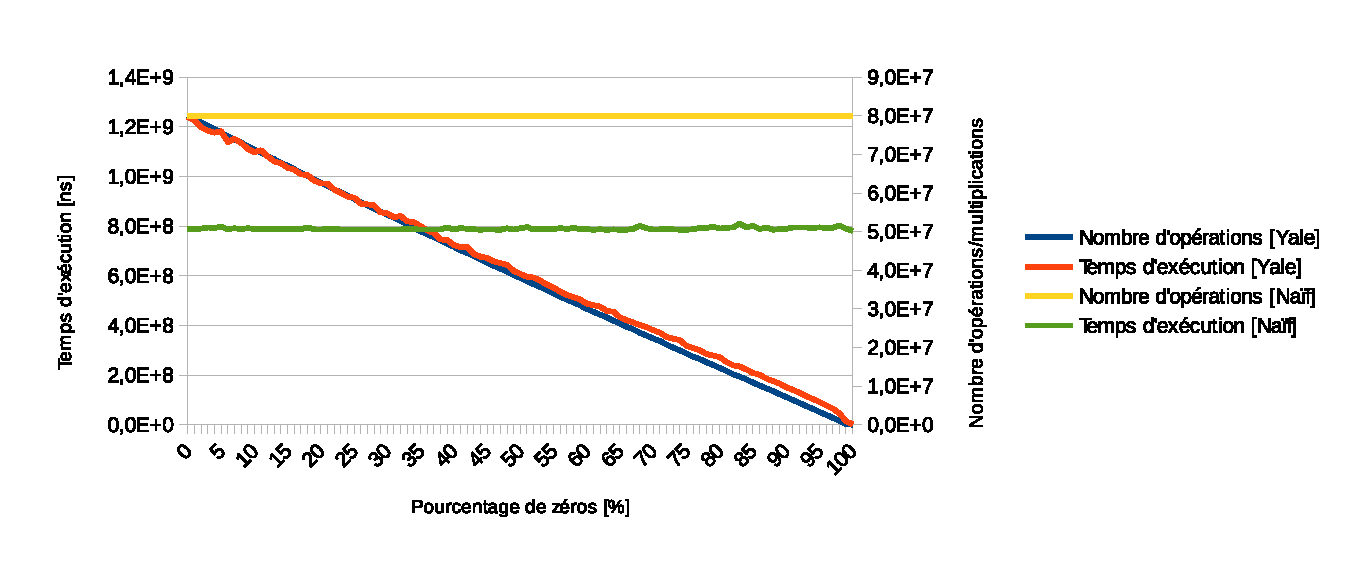
\includegraphics[scale=0.75]{graphe.eps}
\caption{Temps d'exécution et nombre d'opérations pour les deux représentations}
\label{graphe}
\end{figure}

Il est évident que la méthode naïve aura toujours un temps d'exécution et un nombre d'opérations plus ou moins constant, puisqu'aucun produit inutile n'est évité, et que la taille des matrices, est, dans ce cas, toujours la même.

On constate que la méthode optimisée est plus lente pour des matrices en dessous de 40\% de valeurs nulles. Ce phénomène peut notamment s'expliquer par le fait que la représentation de Yale s'avère plus lourde que la représentation classique si l'on considère des matrices pleines (étant donné que les positions des valeurs sont retenues dans le premier cas). La méthode n'est effectivement conçue que pour des matrices ayant une grande quantité de valeurs nulles.

Un dernier constat est que le temps d'exécution et le nombre d'opérations diminuent linéairement par rapport au pourcentage de valeurs nulles contenues dans la matrice.

\section{Conclusion}
Ce projet nous a permis de mettre en pratique une méthode de résolution de problème très pratique en ingénierie. Il nous a également permis de rafraîchir nos connaissances en C et particulièrement dans la manipulation des pointeurs et des fichiers.

En raison d'un timing écourté par nos emplois du temps, nous n'avons pas préféré entamer la réalisation de la parallélisation, telle que proposée en bonus.
\end{document}
